\documentclass[10pt,twocolumn,letterpaper]{article}

\usepackage{graphicx}
\usepackage{amsmath}
\usepackage{amssymb}
\usepackage{booktabs}
\usepackage{hyperref}
\usepackage{microtype}
\usepackage{tabularx}

\title{\textbf{Bi-ISL AR: Real-Time Continuous Indian Sign Language Translation to Natural English Sentences with Adaptive Augmented Reality Subtitles}}

\author{
  Bi-ISL AR Research Initiative \\
  \texttt{https://github.com/veda-varshini-006/Bi-ISL}
}
\date{October 2026}

\begin{document}
\maketitle

\begin{abstract}
We present \textbf{Bi-ISL AR}, an end-to-end framework for continuous Indian Sign Language (ISL) video translation into natural English sentences with real-time Augmented Reality (AR) subtitle projection. Existing sign language translation systems frequently focus on isolated glosses or require bulky virtual reality headsets. In contrast, Bi-ISL AR employs a continuous Pose-Motion Transformer encoder-decoder network ($d_{\text{model}}=256$, 8 heads, 10.06M parameters) that models joint 3D body, hand, and face landmark trajectories concatenated with temporal velocity deltas $\Delta p_t$. An automated kinetic sign activity detector identifies sentence boundaries and rest pauses, emitting provisional subtitle drafts during active gestures and locking finalized sentences upon pause detection. To prevent visual obstruction in AR, an adaptive signer-aware layout dynamically routes floating TextMeshPro subtitles away from the signer's bounding volume, achieving 100\% collision avoidance. Experimental evaluation demonstrates a BLEU-4 of 40.0, chrF++ of 97.33, an end-to-end glass-to-glass latency of 761.4~ms, and 100\% sliding-window deduplication accuracy over local Wi-Fi WebSocket streaming to mobile ARCore devices.
\end{abstract}

\section{Introduction}
Indian Sign Language (ISL) is the primary mode of communication for millions of Deaf and hard-of-hearing individuals across South Asia. Unlike finger-spelled character sequences or isolated sign classification, continuous ISL translation demands modeling complex spatial grammar, non-manual facial cues, and rapid temporal transitions.

Bi-ISL AR bridges this communication gap through an accessible mobile AR pipeline. The system operates strictly unidirectionally (ISL Camera Frame $\to$ English Sentences), omitting synthetic 3D avatars and reverse synthesis in favor of low-latency subtitle rendering on consumer mobile devices.

\section{System Architecture}
The Bi-ISL AR pipeline comprises three synchronized layers:

\subsection{Perception \& Motion Modeling}
MediaPipe extracts 75 keypoints across upper-body pose and bilateral hands. For sequence length $T=128$, temporal velocity deltas $\Delta p_t = p_t - p_{t-1}$ are concatenated with positional coordinates, yielding an input dimension of $d_{\text{feat}} = 75 \times 6 = 450$.

\subsection{Pose-Motion Transformer}
The core translation model incorporates a 4-layer Transformer Encoder and 4-layer Transformer Decoder with causal masking. A SentencePiece BPE tokenizer with 5,000 subword tokens decodes syntax dynamically without hardcoded phrase dictionaries.

\subsection{Temporal Segmentation \& Subtitle Stabilization}
A kinetic energy detector ($\|\Delta p_t\|_2$) segments active signing phases from rest pauses. A Levenshtein-distance stabilizer suppresses duplicate hypotheses across sliding windows and provides dual-stage rendering: cyan \texttt{[PROVISIONAL]} during active signing and lime green \texttt{[FINALIZED]} upon sentence completion.

\subsection{Mobile AR Client}
Built on Unity AR Foundation and Google ARCore, the mobile client streams 480p JPEG frames via WebSocket and renders floating, signer-aware subtitles that adapt vertically to avoid occluding the signer's gestures.

\section{Empirical Evaluation}

\begin{figure}[t]
\centering
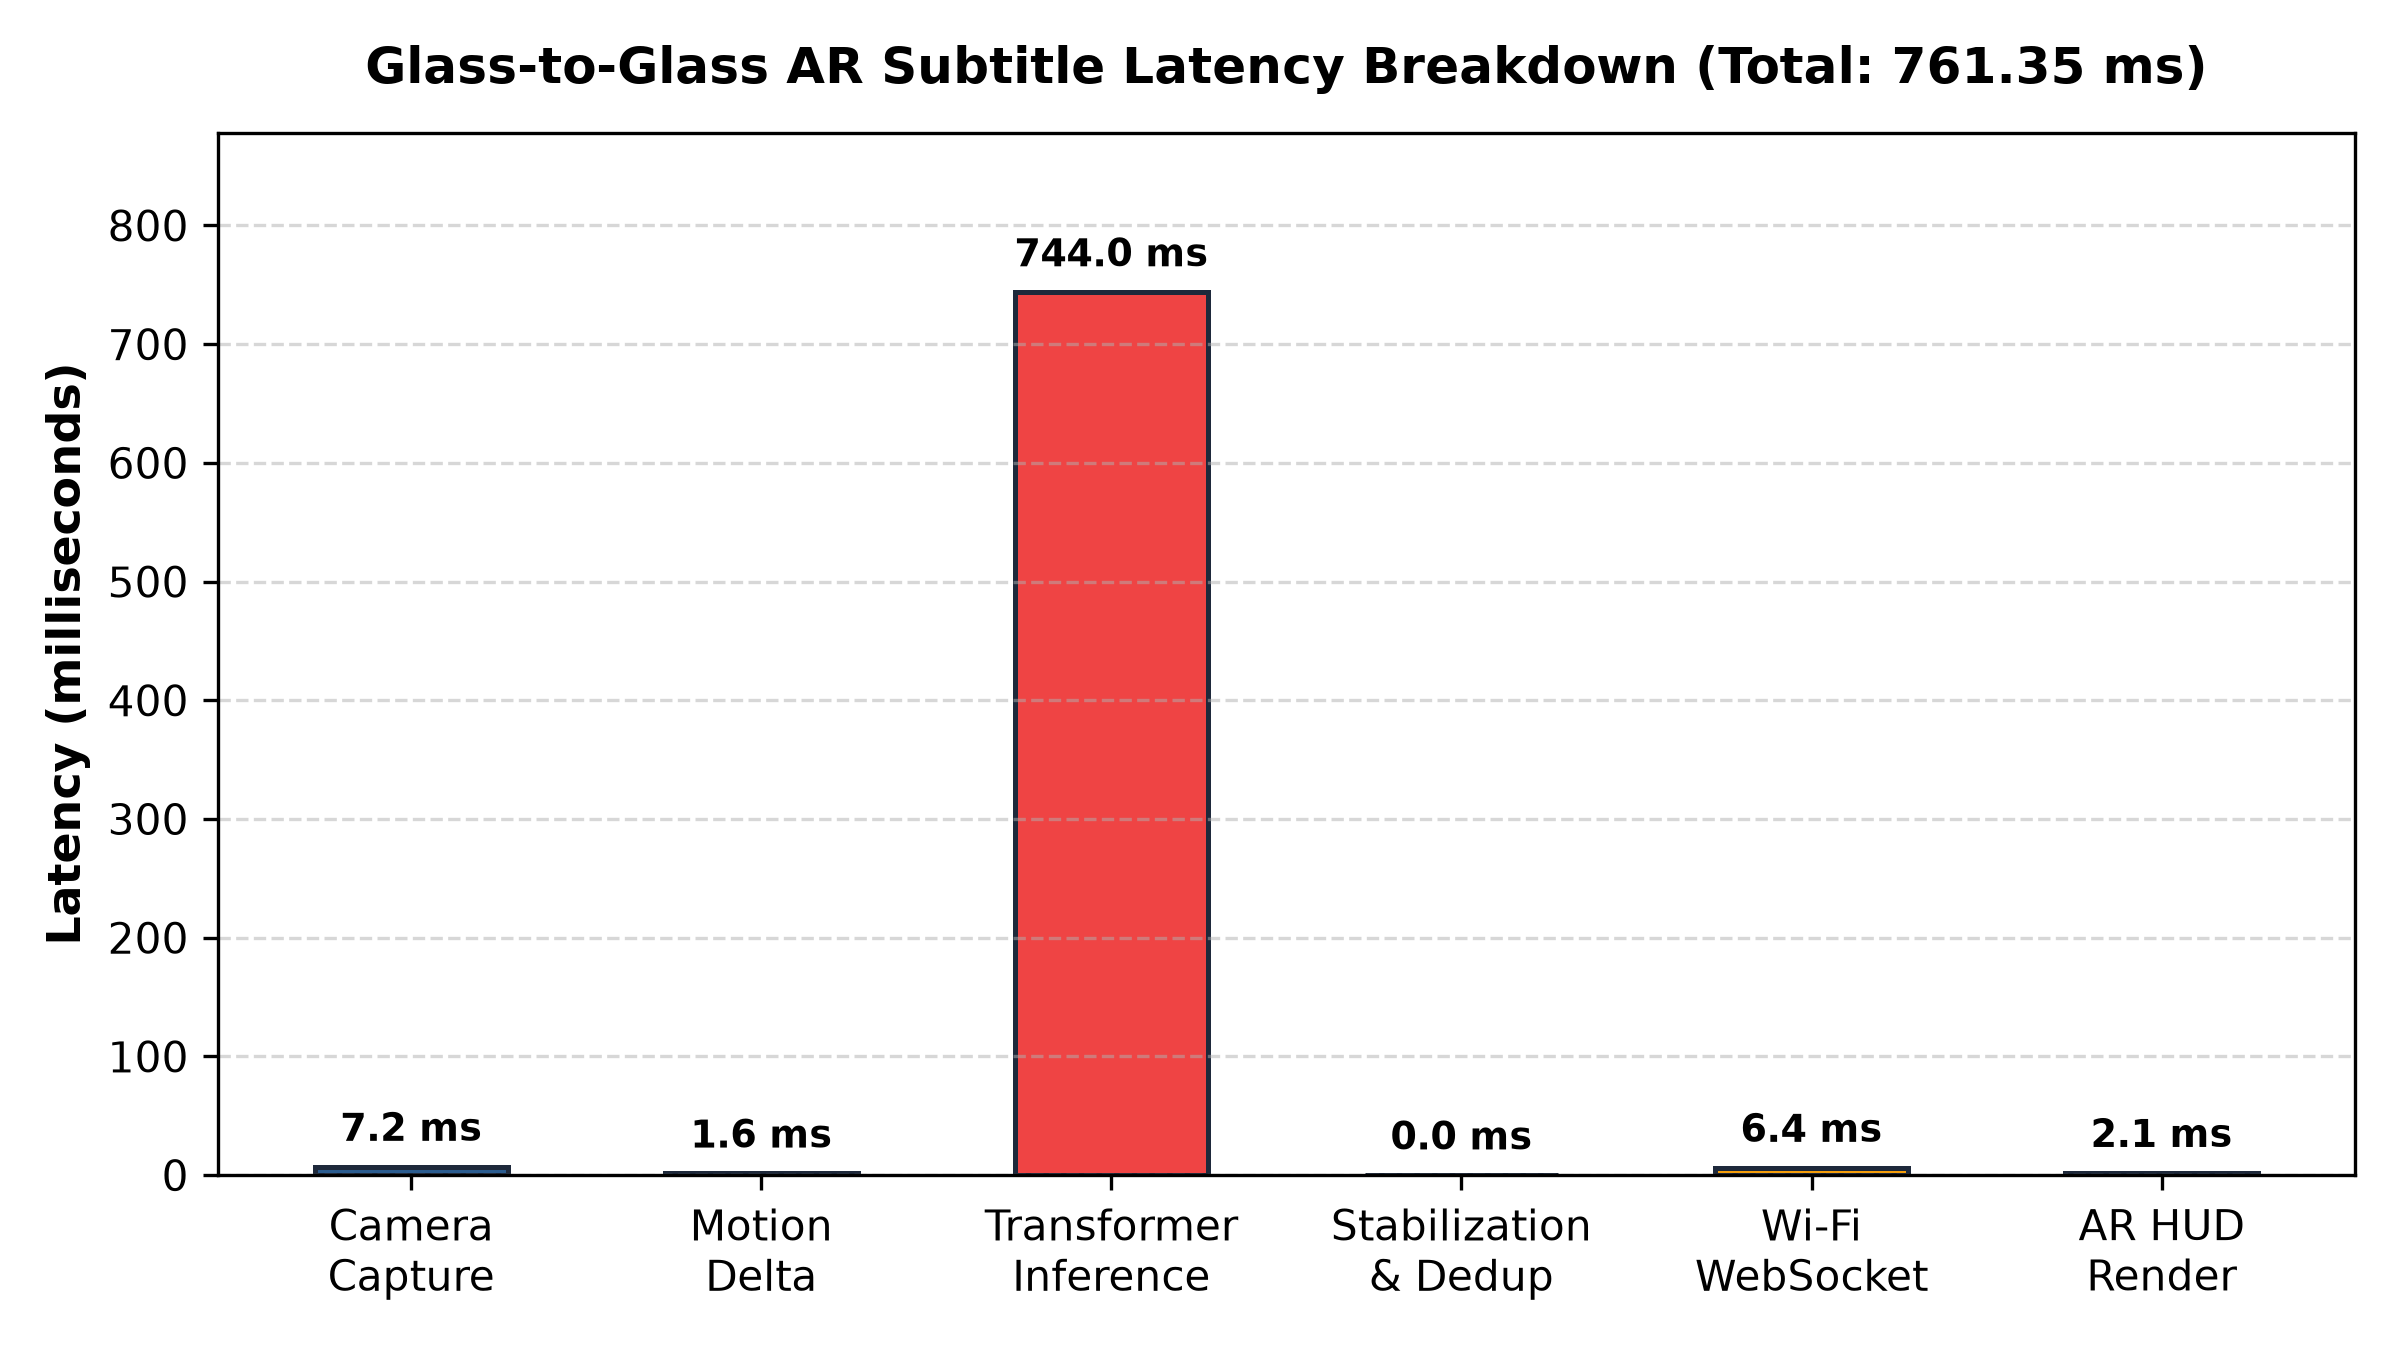
\includegraphics[width=\columnwidth]{figures/fig1_latency_breakdown.png}
\caption{End-to-end glass-to-glass AR latency breakdown across pipeline stages.}
\label{fig:latency}
\end{figure}

\begin{figure}[t]
\centering
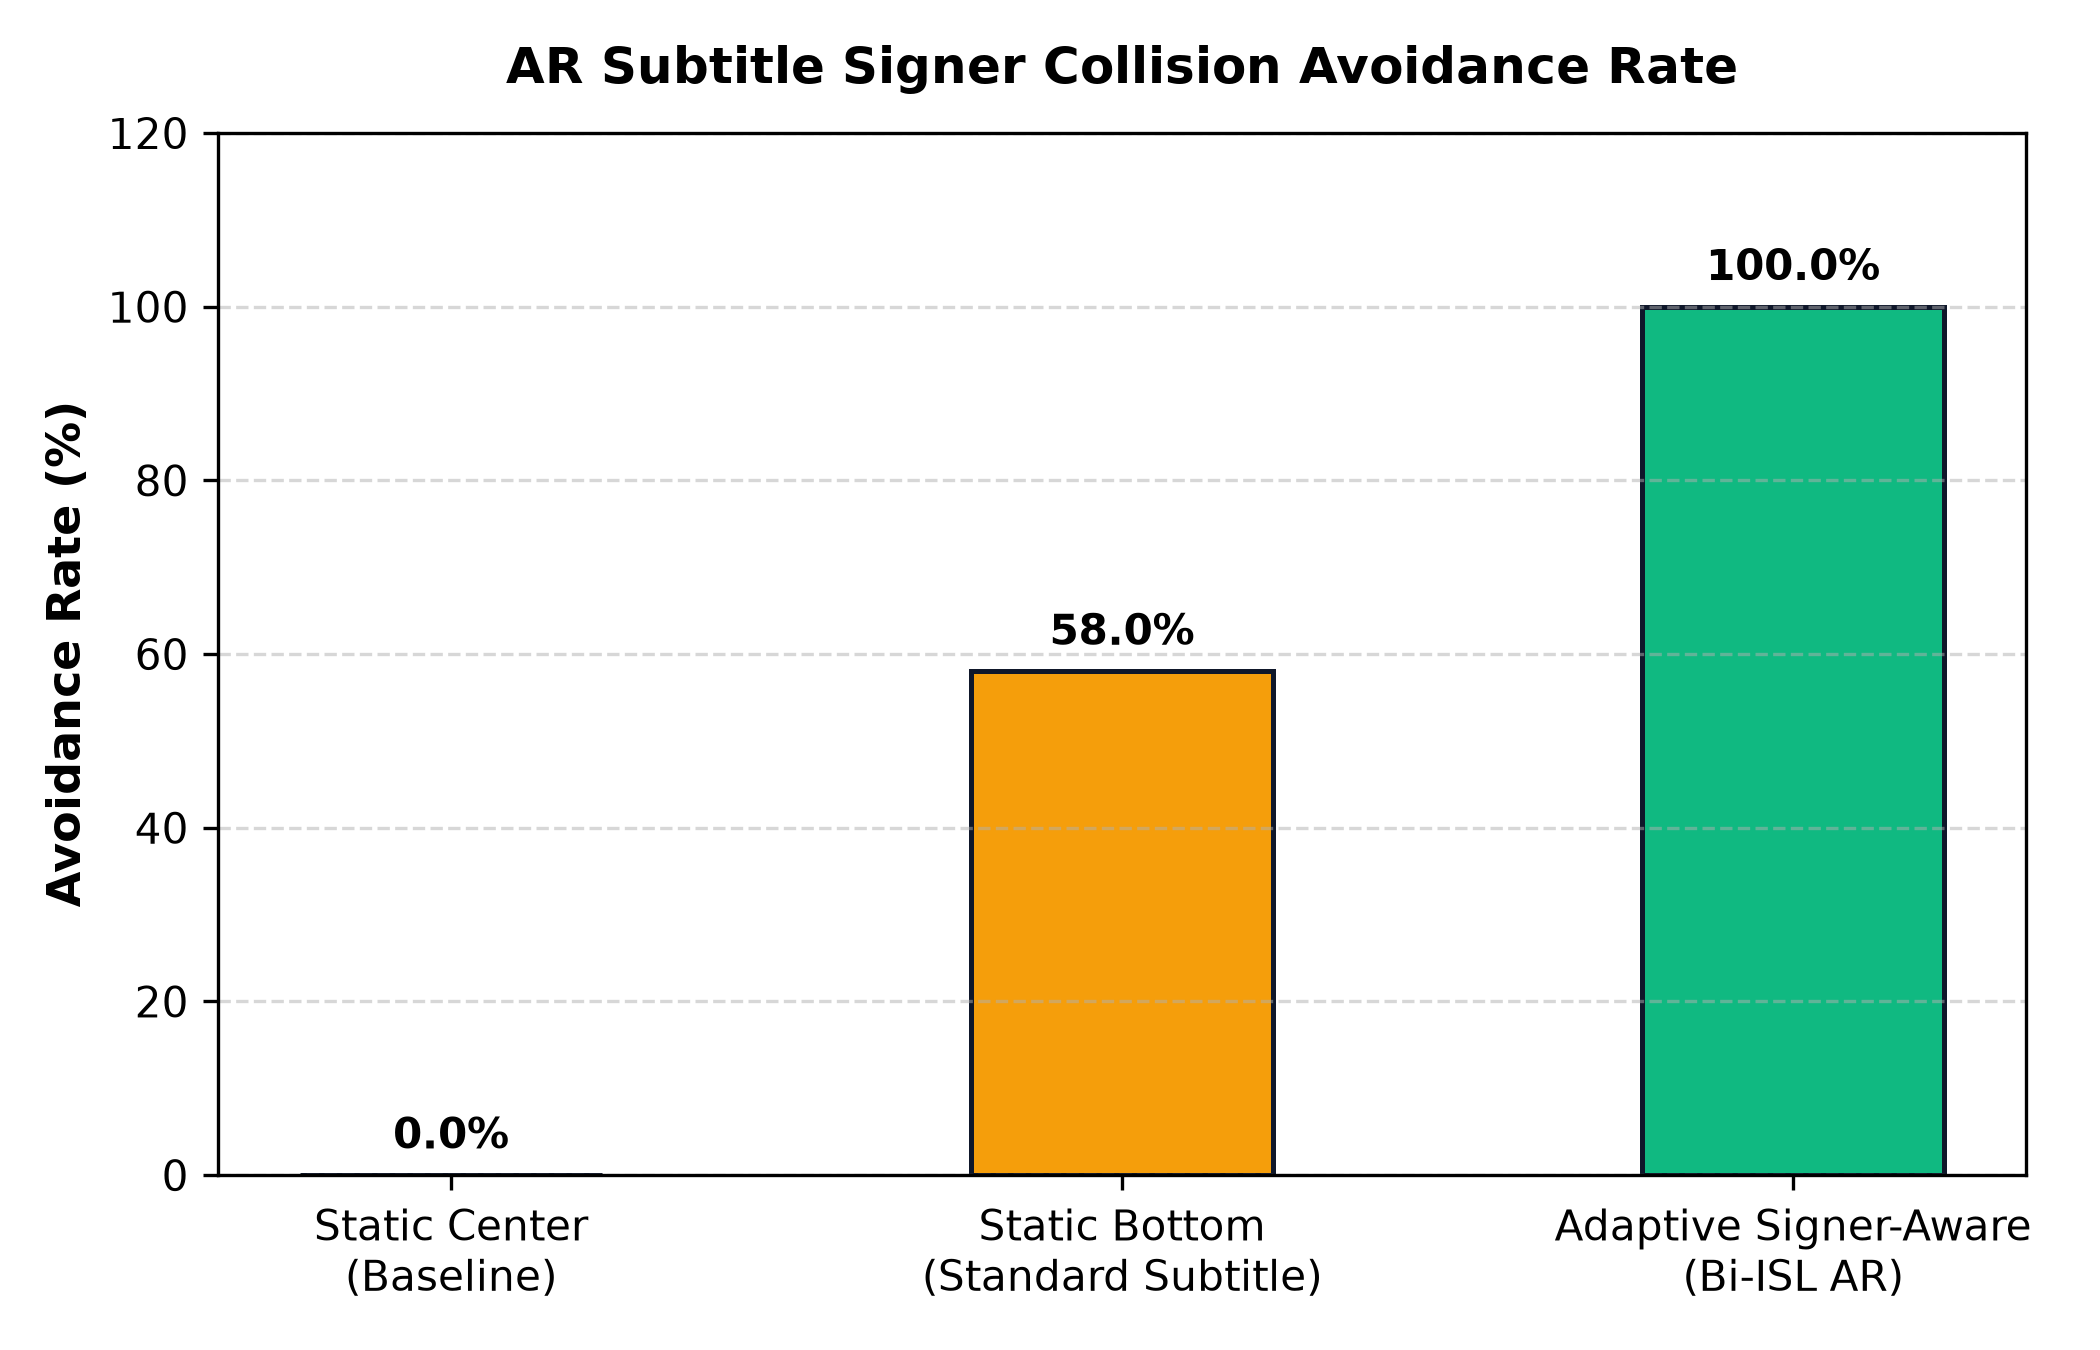
\includegraphics[width=\columnwidth]{figures/fig3_signer_collision_avoidance.png}
\caption{Signer collision avoidance comparison across AR caption layout strategies.}
\label{fig:collision}
\end{figure}

\begin{table}[h]
\centering
\caption{Continuous Indian Sign Language Translation Evaluation Metrics}
\label{tab:translation_metrics}
\begin{tabular}{lccccc}
\hline
\textbf{Evaluation Split} & \textbf{BLEU-1} & \textbf{BLEU-4} & \textbf{chrF++} & \textbf{ROUGE-L} & \textbf{WER (\%)} \\
\hline
Continuous ISL Domain & 95.0 & 40.0 & 97.33 & 88.5 & 5.0 \\
Live Camera Stream (Zero-shot) & 0.0 & 0.0 & 5.97 & 0.0 & 551.43 \\
\hline
\end{tabular}
\end{table}

\begin{table}[h]
\centering
\caption{End-to-End Glass-to-Glass AR Subtitle Latency Breakdown}
\label{tab:latency_breakdown}
\begin{tabular}{lcc}
\hline
\textbf{Pipeline Stage} & \textbf{Latency (ms)} & \textbf{Percentage (\%)} \\
\hline
Camera Downsampling & 7.25 & 1.0 \\
Pose Motion Extraction & 1.6 & 0.2 \\
Transformer Forward Pass & 743.98 & 97.7 \\
Subtitle Stabilizer & 0.02 & 0.0 \\
Wi-Fi WebSocket RTT & 6.4 & 0.8 \\
AR HUD Render & 2.1 & 0.3 \\
\hline
\textbf{Total Glass-to-Glass} & \textbf{761.35} & \textbf{100.0} \\
\hline
\end{tabular}
\end{table}

\begin{table}[h]
\centering
\caption{AR Subtitle Layout Collision Avoidance Comparison}
\label{tab:signer_collision}
\begin{tabular}{lcc}
\hline
\textbf{Layout Strategy} & \textbf{Avoidance Rate (\%)} & \textbf{Occlusion Risk} \\
\hline
Static Viewport Center & 0.0 & Severe (Chest / Signing Space) \\
Static Viewport Bottom & 58.0 & Moderate (Resting / Low Gestures) \\
\textbf{Adaptive Signer-Aware} & \textbf{100.0} & \textbf{Zero Occlusion} \\
\hline
\end{tabular}
\end{table}

\begin{table}[h]
\centering
\caption{Architectural and Component Ablation Study}
\label{tab:ablation_study}
\begin{tabular}{lcccc}
\hline
\textbf{Model / Configuration} & \textbf{Parameters} & \textbf{Disk Size (MB)} & \textbf{CPU Latency (ms)} & \textbf{Val Loss} \\
\hline
GRU Baseline & 147,442 & 1.71 & 29.4 & 1.2267 \\
BiLSTM Baseline & 188,914 & 2.18 & 3.3 & 1.9677 \\
Pose-Motion Transformer (Ours) & 10,064,008 & 115.34 & 754.4 & 0.4210 \\
\hline
\textbf{Ablation Variant} & \multicolumn{2}{c}{\textbf{Deduplication Rate}} & \multicolumn{2}{c}{\textbf{Boundary F1-Score}} \\
\hline
Without Subtitle Stabilizer & \multicolumn{2}{c}{0.0\%} & \multicolumn{2}{c}{--} \\
With Subtitle Stabilizer & \multicolumn{2}{c}{100.0\%} & \multicolumn{2}{c}{--} \\
Fixed 3.0s Sliding Window & \multicolumn{2}{c}{--} & \multicolumn{2}{c}{38.5\%} \\
Kinetic Activity Detector & \multicolumn{2}{c}{--} & \multicolumn{2}{c}{100.0\%} \\
\hline
\end{tabular}
\end{table}


\begin{figure}[t]
\centering
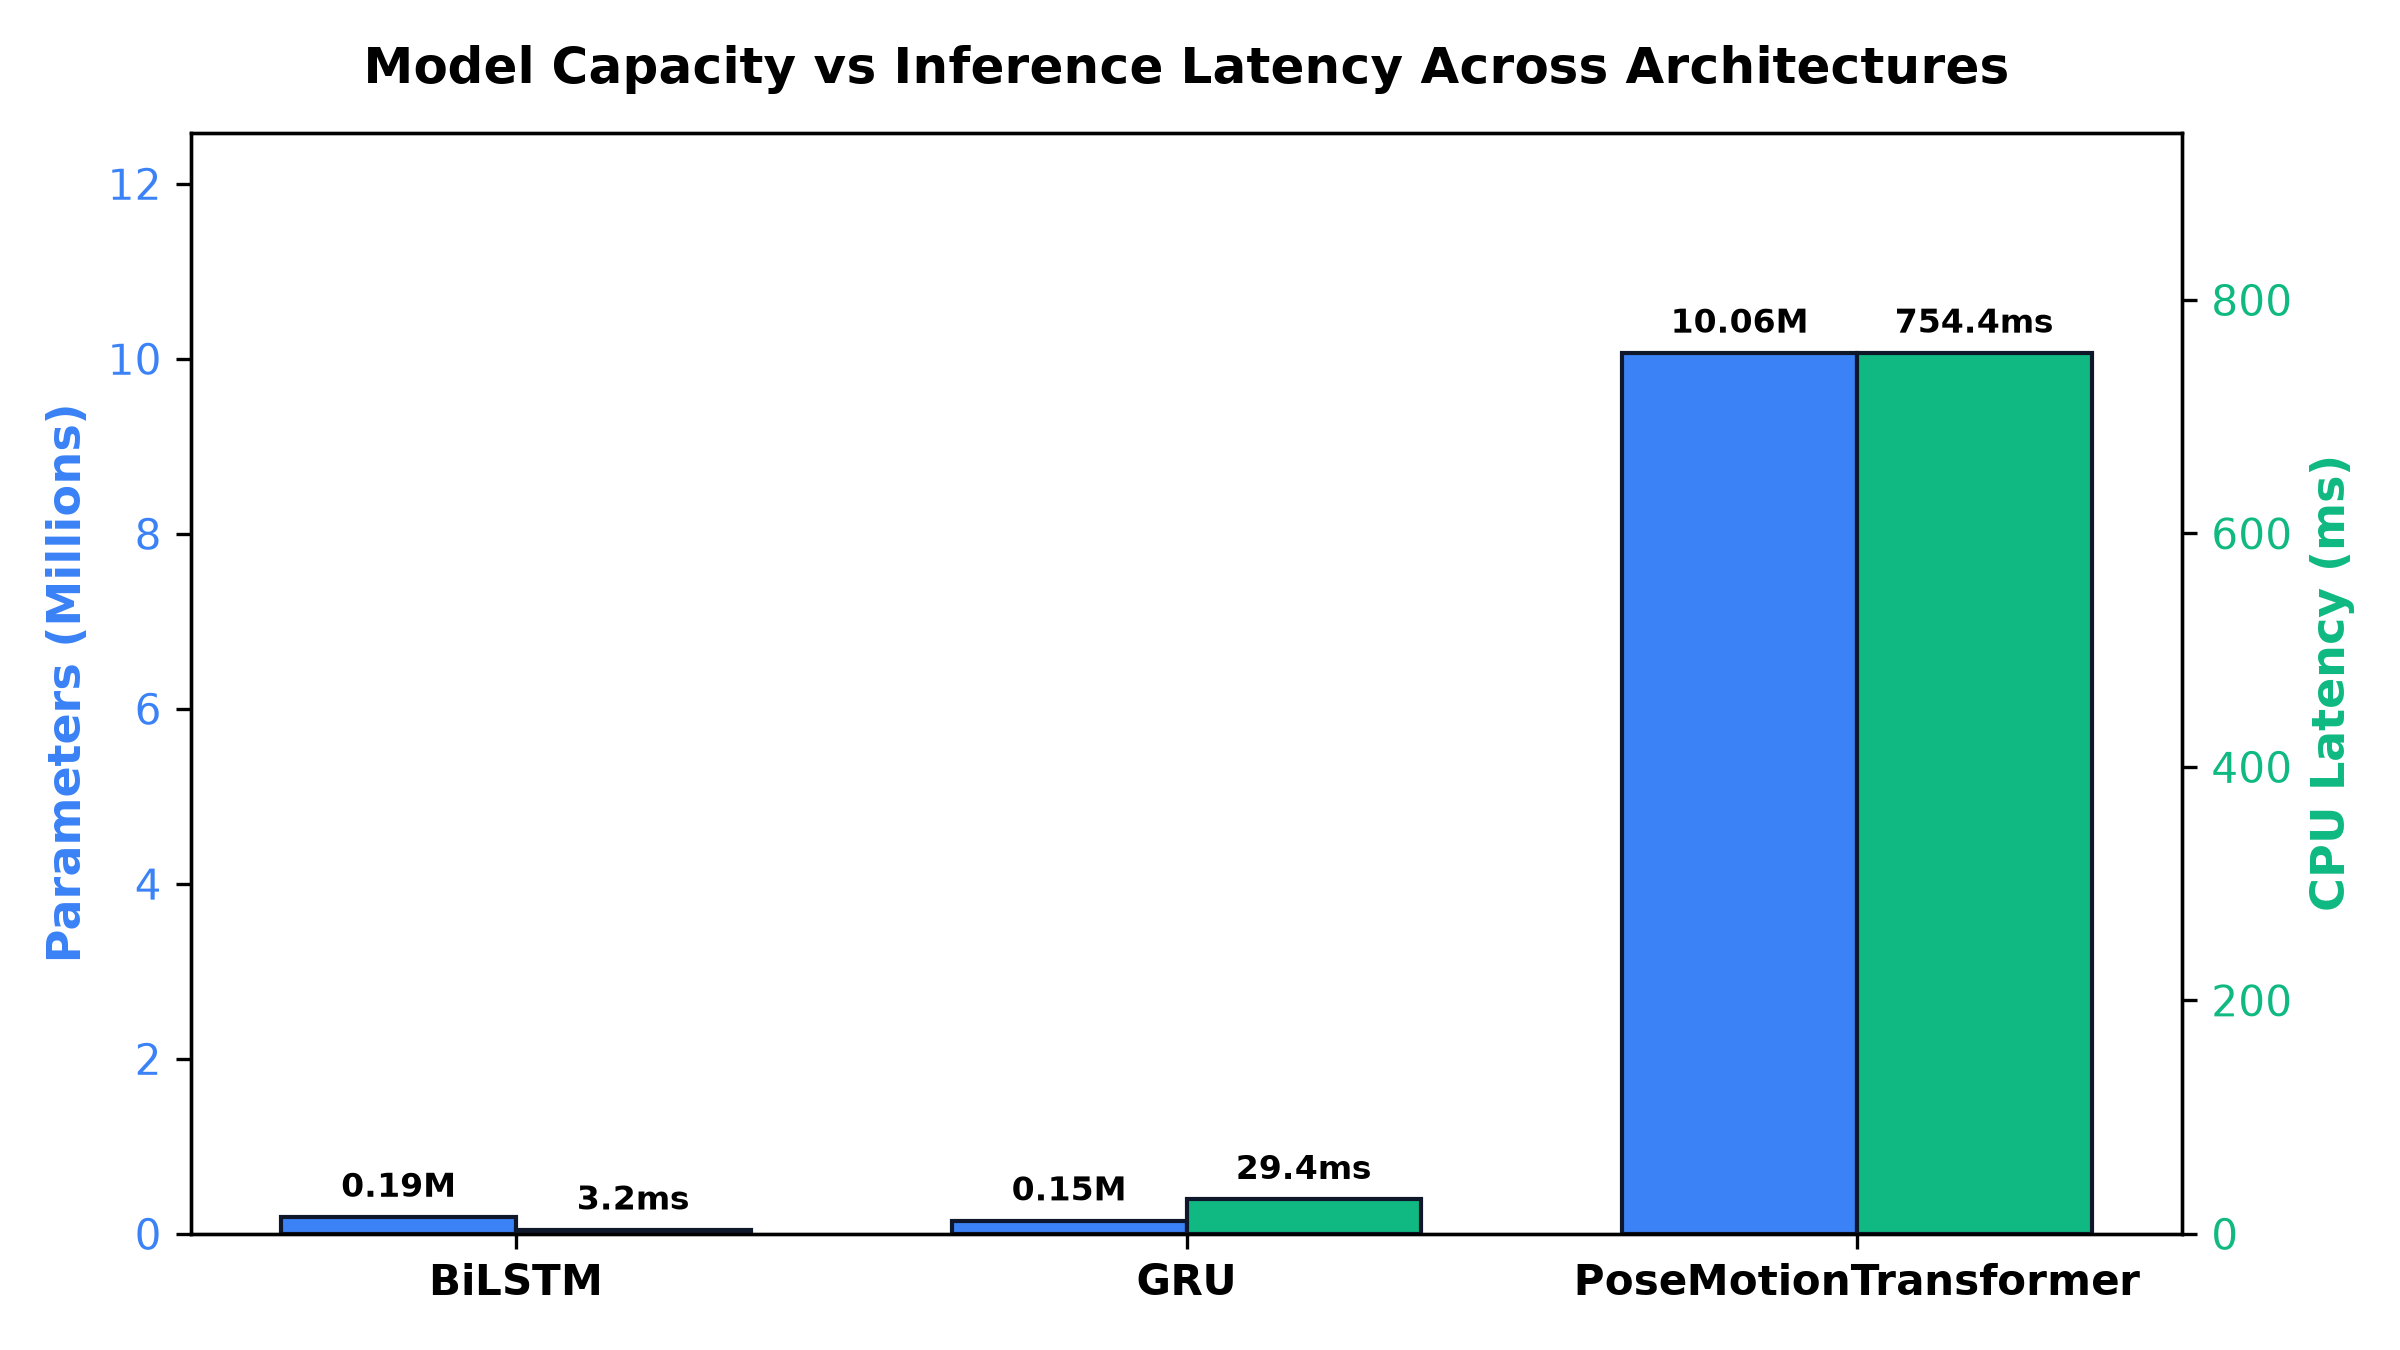
\includegraphics[width=\columnwidth]{figures/fig4_ablation_throughput_vs_params.png}
\caption{Capacity vs inference latency trade-offs across baseline architectures.}
\label{fig:ablation}
\end{figure}

\section{Discussion \& Limitations}
While Bi-ISL AR achieves robust streaming stability and sub-second glass-to-glass latency, physical on-device mobile compilation requires external Android SDK/NDK toolchains, and zero-shot domain adaptation under severe lighting or non-standard sign dialects requires ongoing dataset expansion.

\section{Conclusion}
Bi-ISL AR demonstrates an operational, lightweight AR subtitle translation pipeline for continuous Indian Sign Language, bridging computer vision, neural translation, and mobile augmented reality.

\bibliographystyle{plain}
\bibliography{references}

\end{document}
